\section{Introdução} % Seções são adicionadas para organizar sua apresentação em blocos discretos, todas as seções e subseções são automaticamente exibidas no índice como uma visão geral da apresentação, mas NÃO são exibidas como slides separados.

%------------------------------------------------

\begin{frame}
    \frametitle{Introdução à Machine Learning}
    
    Processo de ensinar um computador a fazer previsões ou tomar decisões a partir de dados, identificando padrões ou regularidades.

    \vspace{0.5cm}

    \textbf{Exemplos:}
    \begin{enumerate}
        \setlength{\itemsep}{10pt}
        \item Recomendação de Produtos (ex.: Netflix, Amazon)
        \item Reconhecimento de Imagens (ex.: diagnóstico médico, reconhecimento facial)
        \item Previsão de Séries Temporais (ex.: previsão de demanda, previsão de vendas)
    \end{enumerate}
\end{frame}

\begin{frame}
	\frametitle{Introdução à Machine Learning}
    \vspace{0.2cm}
     \textbf{Fluxo de Trabalho}
     \vspace{0.2cm}
    \begin{itemize}
        \item Pré Processamento
        \item Treinamento
        \item Validação
    \end{itemize}
     
    \begin{center}
        \centering
        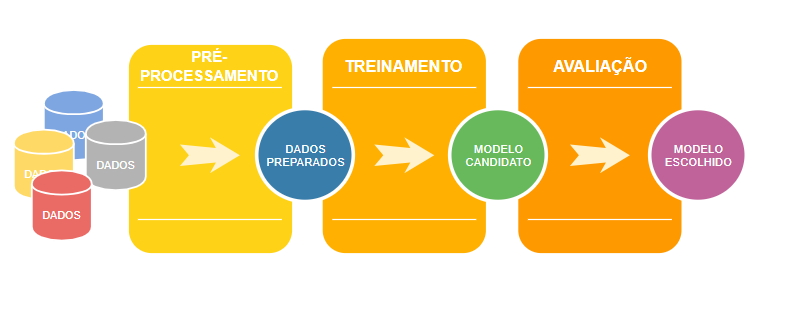
\includegraphics[width=1.0\linewidth]{img/introaml.png}
    \end{center}
\end{frame}

\begin{frame}
    \frametitle{Desenvolvimento no Colab}
    \centering
    
    Link para o acesso ao minicurso no colab\\ está no site do GET-EngComp:

    \vspace{0.5cm}
    
    \href{https://www2.ufjf.br/getengcomp/}{www2.ufjf.br/getengcomp/}        
\end{frame}